\chapter{Google APIs}\label{ch:google_api}

Se conoce por este nombre al conjunto de \glspl{API} desarrolladas por Google y que permiten a aplicaciones de terceros acceder a los servicios de Google, como pueden ser Search, Google Map, Google Traslator, Gmail, \ldots. El uso de estas \glspl{API} suelen estar limitado a un número de peticiones diarias, acarreando un coste adicional todas aquellas que superen este límite.

Para poder hacer uso de estas \glspl{API} es necesario autorización y autenticación, es por ello necesario crear antes una cuenta en Google para poder obtener las credenciales con las que autenticarnos ante los servicios de Google. Si ya disponemos de una cuenta en Google, podremos acceder a la consola para desarrolladores\footnote{\url{https://console.developers.google.com}}. Desde esta consola podremos realizar diferentes gestiones sobre nuestra cuenta.

\begin{figure}[H]
\centering
  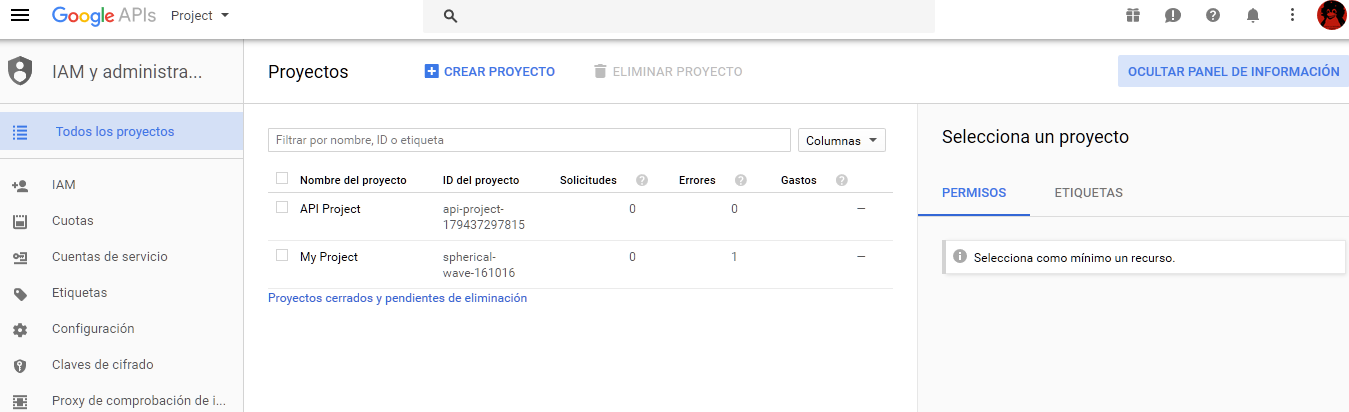
\includegraphics[width=0.8\textwidth]{Figures/anexo/google_api/developer_console}
  \caption{Consola para desarrolladores de Google.}
\end{figure}

A nuestra cuenta le podemos asignar varios proyectos. Esto nos ayudará a gestionar por separado las credenciales que generemos y poder diferenciar el uso que se le ha dado a cada una de ellas (consumo, número de peticiones, acceso a servicios, \ldots). Esto es útil en caso de tener varias aplicaciones, o simplemente tener una sola aplicación, pero varios entornos (desarrollo, preproducción, producción, piloto, \ldots)

\section{Obtención de una clave para utilizar Google Maps}

Para la realización de una de las prácticas propuestas, va a ser necesario el uso de una clave, \emph{API KEY}, que permita a nuestra aplicación hacer uso del servicio de Google Maps. Vamos a ver como podemos conseguir esta clave. Daremos por supuesto que disponemos de una cuenta de Google a la cual vincularemos nuestro proyecto.

\warningbox{
  Tened en cuenta que el uso de estas \glspl{API} pueden incurrir en costes que serán cargados a la cuenta a la que este asociado el proyecto. Debemos ser cautelosos con el uso que hacemos des de estas claves, y en caso de no necesitarlas, destruirlas.
}

En primer lugar, crearemos un proyecto dentro de nuestra cuenta. Le asignaremos un nombre para poder identificarlo, y si lo deseamos, podremos modificar el ID que asigna Google automáticamente.

\begin{figure}[H]
\centering
  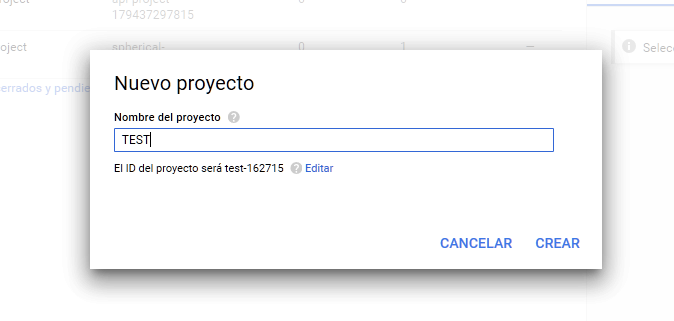
\includegraphics[width=0.8\textwidth]{Figures/anexo/google_api/create_project}
  \caption{Ventana para la creación de un proyecto dentro de nuestra cuenta.}
\end{figure}

Una vez creado, podremos verlo en la lista con el resto de proyectos y podremos seleccionarlo.

\begin{figure}[H]
\centering
  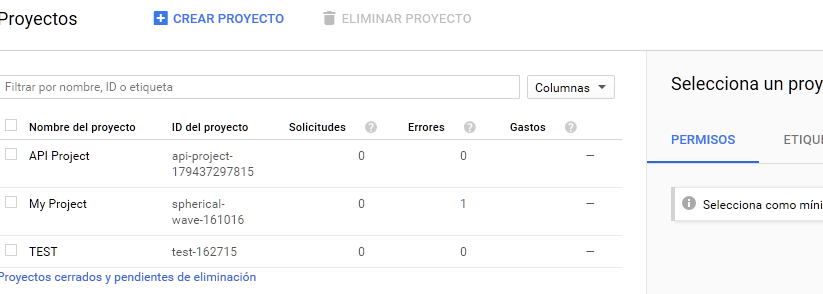
\includegraphics[width=0.8\textwidth]{Figures/anexo/google_api/project_list}
  \caption{Lista de proyectos asociados a nuestra cuenta.}
\end{figure}

Si desplegamos el menú lateral, podremos ver diferentes secciones relativas a nuestro proyecto, dentro de estas secciones a su vez nos encontraremos diferentes apartados, de los cuales, veremos los más importantes.

\begin{figure}[H]
\centering
  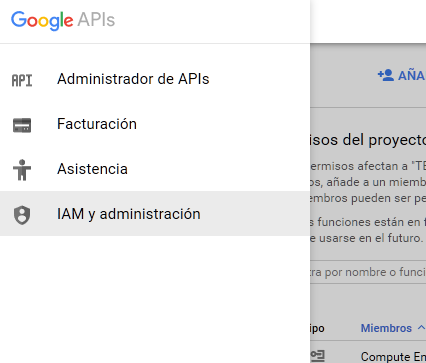
\includegraphics[width=0.6\textwidth]{Figures/anexo/google_api/menu_console}
  \caption{Menú desde el que acceder a diferentes secciones relativas al proyecto.}
\end{figure}

Si accedemos a la sección \textbf{Administrador de APIs}, podremos ver el \textbf{Panel de control}. En este panel aparecerán las estadísticas de uso de los diferentes servicios asociados. Recién creado el proyecto, esta pantalla debería aparecer vacía. Si abrimos la \textbf{Biblioteca}, veremos una lista con los diferentes servicios de Google. Aqui seleccionaremos los servicios que queremos habilitar para nuestro proyecto.

\begin{figure}[H]
\centering
  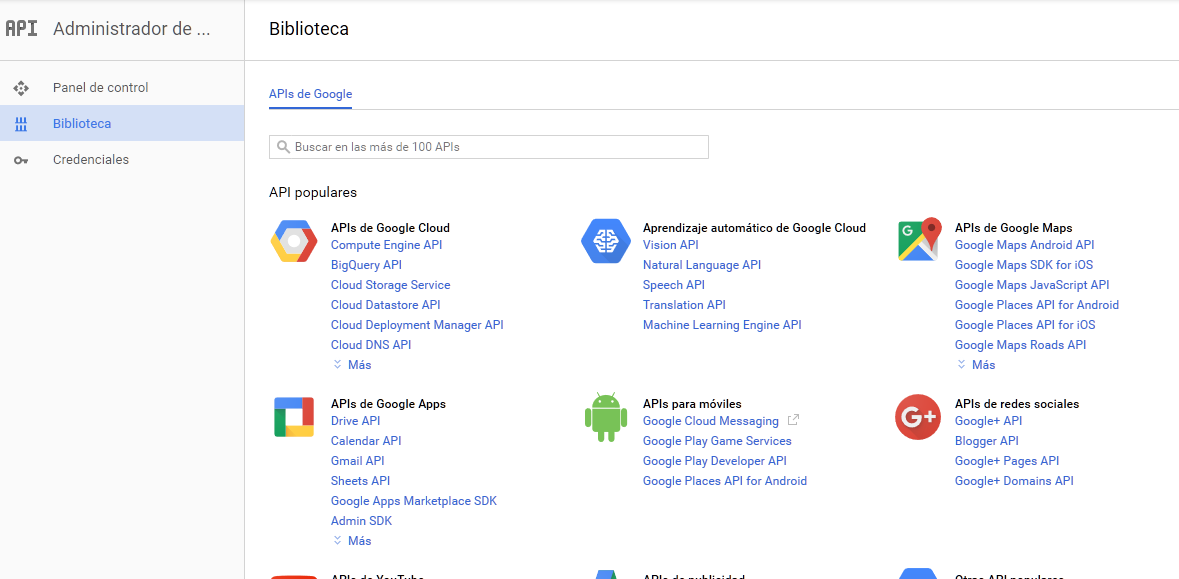
\includegraphics[width=0.8\textwidth]{Figures/anexo/google_api/api_library}
  \caption{APIs disponibles para poder asignar al proyecto.}
\end{figure}

A nosotros nos interesa el servicio \textbf{Google Maps Android API}. Lo seleccionamos y nos aparecerá una pantalla con una pequeña explicación del servicio y un botón con el que habilitarlo.

\begin{figure}[H]
\centering
  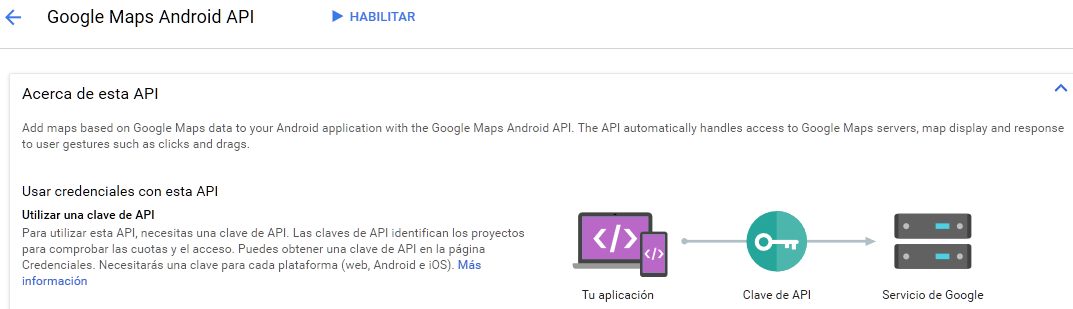
\includegraphics[width=0.8\textwidth]{Figures/anexo/google_api/api_google_map}
  \caption{Información relativa a la API de Google Maps Android.}
\end{figure}

Tras ello nos abrirá de nuevo el panel de control, esta vez, podremos ver las gráficas que nos ofrecen, que aun estando vacías, podremos hacernos una idea de la información que ofrecerán.

El siguiente paso será crear nuestra clave. Lo podremos apartado \textbf{Credenciales}, en la que veremos que al crear una, nos ofrecerá varias opciones, entre ellas, la de generar una clave que es la que nos interesa.

\begin{figure}[H]
\centering
  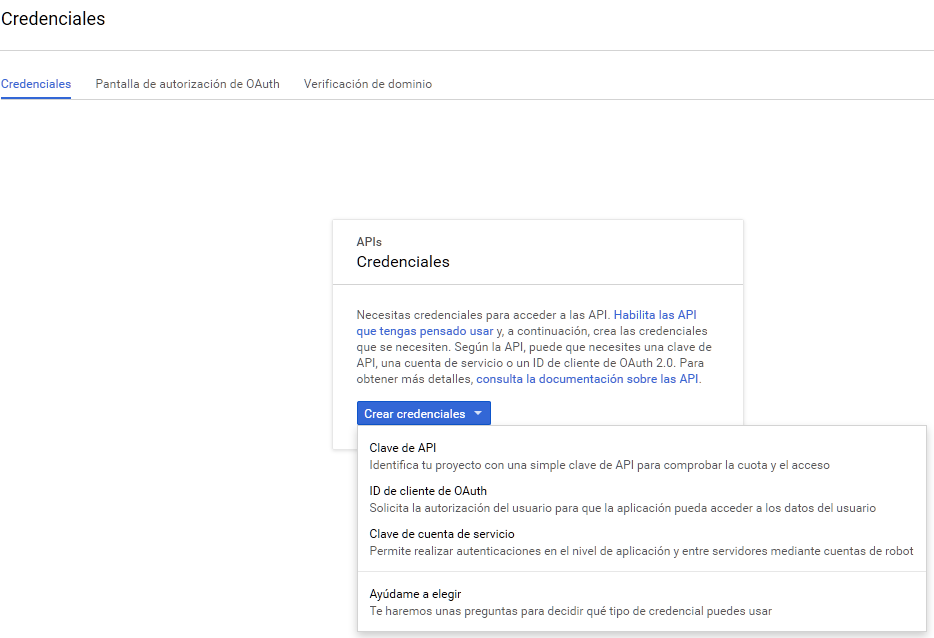
\includegraphics[width=0.8\textwidth]{Figures/anexo/google_api/api_credential}
  \caption{Configuración de las credenciales para nuestra API. El servicio nos proporciona diferentes maneras para realizar la autorización.}
\end{figure}

Una vez creada, nos aparecerá para poder copiarla (aunque podremos consultarla cuando queramos desde la consola) y nos dará la opción de restringir el acceso. Esta opción es muy interesante, especialmente una vez puesta en producción, ya que nos permitirá limitar quien hace uso de ella ya sea mediante una dirección \gls{IP}, una URL, el nombre del paquete de una aplicación de Android, \ldots. Si no ponemos esta restricción, alguien podría obtener la clave desde el código (por ejemplo depurando la aplicación) y utilizarla para su propia aplicación cargandonos a nosotros con los costes de uso.

\begin{figure}[H]
\centering
  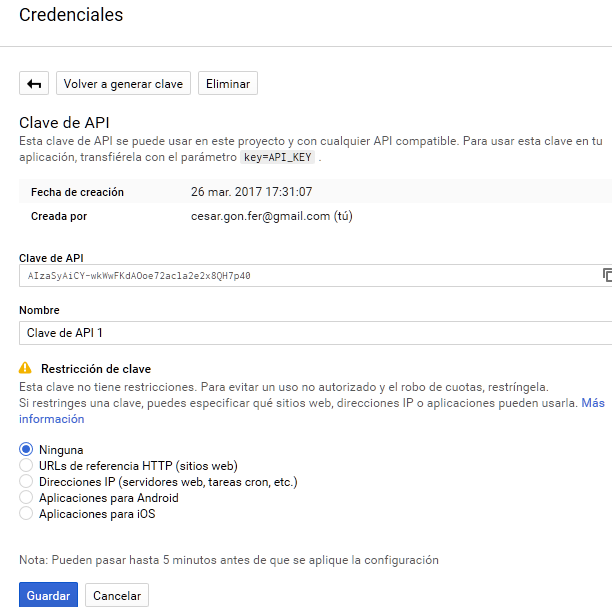
\includegraphics[width=0.7\textwidth]{Figures/anexo/google_api/api_credential_restriction_options}
  \caption{Opciones para restringir el acceso según el origen de la petición. Para una aplicación Android, necesitariamos indicar el nombre del paquete de nuestra aplicación.}
\end{figure}

De vuelta al menú lateral, si nos vamos a la sección \textbf{IAM y administración}, podemos destacar el apartado \gls{IAM}, donde podremos dar permisos sobre el proyecto a otros usuarios, por ejemplo, permisos de edición, de lectura, sobre la facturación, \ldots

\begin{figure}[H]
\centering
  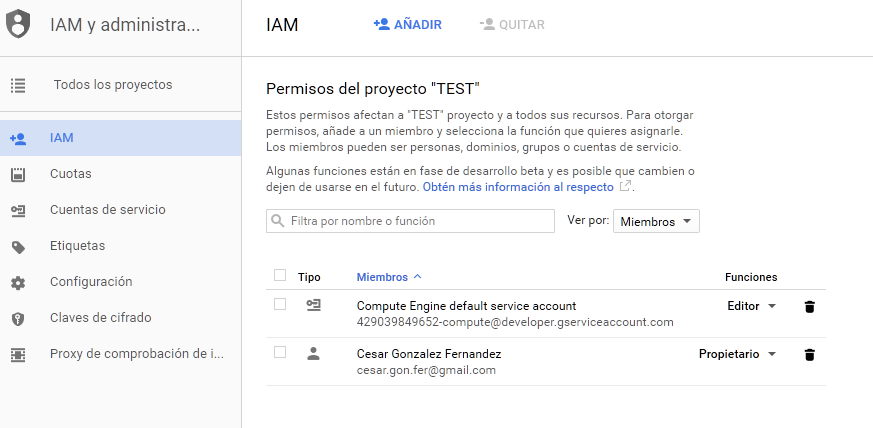
\includegraphics[width=0.8\textwidth]{Figures/anexo/google_api/iam}
  \caption{Permisos sobre el proyecto para distintos usuarios de la consola de desarrolladores. Aquí podemos compartir el proyecto con el resto del equipo de desarrollo y asignarles diferentes permisos a cada uno.}
\end{figure}

Y el apartado de \textbf{Cuotas}, donde vemos las cuotas de los servicios activados y podremos limitarlas.

\begin{figure}[H]
\centering
  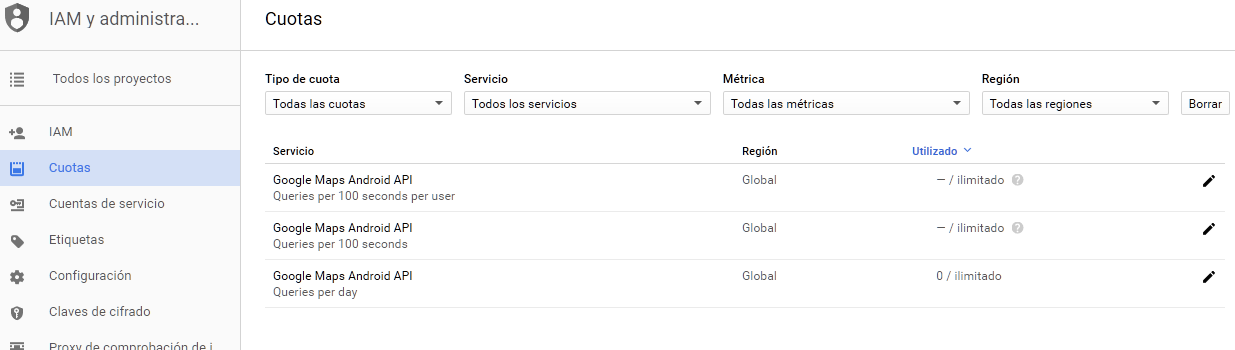
\includegraphics[width=0.8\textwidth]{Figures/anexo/google_api/quota}
  \caption{Cuotas que se aplican a cada uno de los servicios asociados al proyecto.}
\end{figure}
